% Chapter 2

\chapter{Project management} % Main chapter title

\label{Chapter2} % For referencing the chapter elsewhere, use \ref{Chapter1} 

\lhead{Chapter 2. \emph{Project management}} % This is for the header on each page - perhaps a shortened title

%----------------------------------------------------------------------------------------
In this chapter we want to present how our group organized and managed this project. Group members are:
\begin{itemize}
\item Ozan
\item Oksana
\item Klemen
\item Natalia
\end{itemize}
As we all had a bit of experiences in software design, we knew how important a proper plan and research before the actual implementation is. Unfortunately, we were also aware that no matter how good the plan is, we will be forced to adjust it during the implementation. Either because of the things we overlooked while planning or because some assumptions we made were wrong. We decided to follow the \textit{iterative and incremental development model}, which enabled us to adjust our plans after each of the implementation iterations. A schematic representation of the iterative and incremental development model can be seen on figure \ref{fig:Iterative_development_model_V2}.
\begin{figure}[h]
\centering
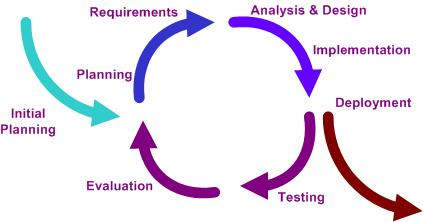
\includegraphics[height=4cm]{../pictures/Iterative_development_model_V2}
\caption{An iterative development model (image taken from \cite{wiki1})}
\label{fig:Iterative_development_model_V2}
\end{figure}

\section{Basic building blocks}
\label{Building blocks}
On our first meeting we decided to split the project into four main parts to be able to fully manage the whole project at all times. This parts are:
\begin{itemize}
\item User interface
\item Database and data structure
\item Map representation
\item Path algorithms
\end{itemize}

\subsection{UI - User Interface}
Part of the application that is responsible for user interaction with the application. Main goal is to make the interface as user-friendly as possible. In the beginning we made a rough sketch of how the interface should look (figure []), which has, as expected, changed during the process of later design and implementation. The UI is presented more in details in chapter [UI USER MAUNAL].
\subsection{Database and data structure}
Our database consists of two parts. The static part, having the information about the roads in Le Creusot (described in []) and the dynamic part with the information about the points of interest (POI). In chapter[] we address the facts we took into account while considering different database options and data structures.
\subsection{Map representation}
We separated map representation from other parts of user interface, because we think it is the most important of UI, so we will give special attention to it.
\subsection{Path algorithms}
In the different algorithms we adopted and developed, we do all the searching for paths, calculating distance and travel times and optimize the search results as much as possible. Our main goal is to make the algorithms work as  quickly as possible, taking into account all the restrictions road networks has (oneway streets, footways etc.). We also want to make the algorithms as reusable as possible, to reduce the redundancy in development and minimize the possibilities of errors.

\section{Softwares used for project management}
Github, skype etc.
\section{Meetings}
some bullshit about that

